% Metódy inžinierskej práce

\documentclass[10pt,twocolumn,twoside,slovak,a4paper]{article}

\usepackage[slovak]{babel}
%\usepackage[T1]{fontenc}
\usepackage{graphicx}
\graphicspath{ {./} }
\usepackage[IL2]{fontenc} % lepšia sadzba písmena Ľ než v T1
\usepackage[utf8]{inputenc}
\usepackage{graphicx}
\usepackage{url} % príkaz \url na formátovanie URL
\usepackage{hyperref} % odkazy v texte budú aktívne (pri niektorých triedach dokumentov spôsobuje posun textu)
\usepackage{subfig}
\usepackage{cite}
\usepackage{amsmath}
\usepackage{wrapfig}
%\usepackage{times}

\pagestyle{headings}

\title{GPU Acceleration for Regular Expressions: Revision on Newer Hardware
\thanks{Semestjrálny projekt v predmete Metódy inžinierskej práce, ak. rok 2023/24, vedenie: MSc. Mirwais Ahmadzai}} % meno a priezvisko vyučujúceho na cvičeniach

\author{Roman Gajdoš\\[2pt]
	{\small Slovenská technická univerzita v adfadfa}\\
	{\small Fakulta informatiky a informačných technológií}\\
	{\small \texttt{...@stuba.sk}}
	}

\date{\small 25. september 2023} % upravte



\begin{document}

\maketitle

\begin{abstract}
	\ldots
\end{abstract}



\section{Úvod}

Motivujte čitateľa a vysvetlite, o čom píšete. Úvod sa väčšinou nedelí na časti.

Uveďte explicitne štruktúru článku. Tu je nejaký príklad.
Základný problém, ktorý bol naznačený v úvode, je podrobnejšie vysvetlený v časti~\ref{nejaka}.
Dôležité súvislosti sú uvedené v častiach~\ref{dolezita} a~\ref{dolezitejsia}.
Záverečné poznámky prináša časť~\ref{zaver}.



\section{Nejaká časť} \label{nejaka}
\section{Nova cast} \label{nejaky label}
Z obr.~\ref{f:rozhod} je všetko jasné.

% \begin{figure*}[tbh]
% 	\centering
% 	%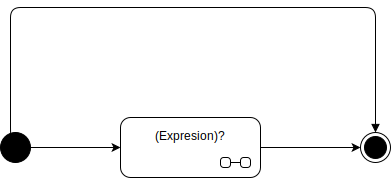
\includegraphics[scale=1.0]{diagram.pdf}
% 	Aj text môže byť prezentovaný ako obrázok. Stane sa z neho označný plávajúci objekt. Po vytvorení diagramu zrušte znak \texttt{\%} pred príkazom \verb|\includegraphics| označte tento riadok ako komentár (tiež pomocou znaku \texttt{\%}).
% 	\caption{Rozhodujúci argument.}
% 	\label{f:rozhod}
% \end{figure*}


\begin{figure*}[htp]
	\centering
	\subfloat[data a]{%
		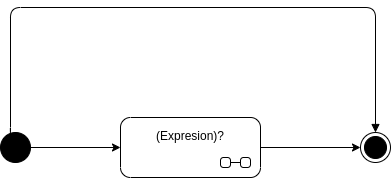
\includegraphics[width=0.4\textwidth]{diagram.png}%
		\label{fig:a}%
	}%
	\hfill%
	\subfloat[data b]{%
		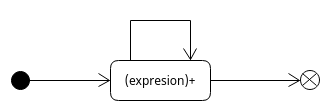
\includegraphics[width=0.4\textwidth]{Diagram2.png}%
		\label{fig:b}%
	}%
	\caption{all the data}
\end{figure*}

% \section{Iná časť} \label{obr1}
% \begin{figure}[t]
% 	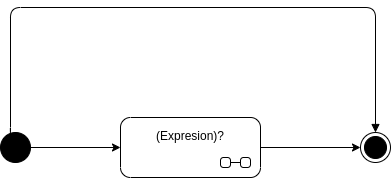
\includegraphics[width=5cm]{diagram.png}
% 	\centering
% 	\caption{Example of state machine diagram of regex expresion '?'}
% \end{figure}

% \section{Iná časť} \label{obr2}
% \begin{figure}[t]
% 	\includegraphics[width=5cm]{diagram2.png}
% 	\centering
% 	\caption{Example of state machine diagram of regex expresion '+'}
% \end{figure}

Základným problémom je teda\ldots{} Najprv sa pozrieme na nejaké vysvetlenie (časť~\ref{ina:nejake}), a potom na ešte nejaké (časť~\ref{ina:nejake}).\footnote{Niekedy môžete potrebovať aj poznámku pod čiarou.}
\begin{wrapfigure}{l}{0.25\textwidth}
	\centering
	
\includegraphics[width=0.25\textwidth]{fiit/PNG/STU-FIIT-anch.png}
\end{wrapfigure}

Môže sa zdať, že problém vlastne nejestvuje\cite{Coplien:MPD}, ale bolo dokázané, že to tak nie je~\cite{Czarnecki:Staged, Czarnecki:Progress}. Napriek tomu, aj dnes na webe narazíme na všelijaké pochybné názory\cite{PLP-Framework}. Dôležité veci možno \emph{zdôrazniť kurzívou}.


\subsection{Nejaké vysvetlenie} \label{ina:nejake}

Niekedy treba uviesť zoznam:

\begin{itemize}
	\item jedna vec
	\item druhá vec
	      \begin{itemize}
		      \item x
		      \item y
	      \end{itemize}
\end{itemize}

Ten istý zoznam, len číslovaný:

\begin{enumerate}
	\item jedna vec
	\item druhá vec
	      \begin{enumerate}
		      \item x
		      \item y
	      \end{enumerate}
\end{enumerate}


\subsection{Ešte nejaké vysvetlenie} \label{ina:este}

\paragraph{Veľmi dôležitá poznámka.}
Niekedy je potrebné nadpisom označiť odsek. Text pokračuje hneď za nadpisom.
$$a_1 + a_2 + a_3 + a_4 + a_5 + a_6 + a_7 + a_8 +a_6 + a_7 + a_8 +a_6 + a_7 + a_8 +a_6 + a_7 + a_8 +a_6 + a_7 + a_8 +a_6 + a_7 + a_8 +\ldots + a_k = \sum_{n=1}^{k} a_n$$

$$\begin{bmatrix}
		x_{11} & x_{12} & x_{13} & x_{14} & x_{15} \\
		x_{21} & x_{22} & x_{23} & x_{24} & x_{25} \\
		x_{31} & x_{32} & x_{33} & x_{34} & x_{35} \\
		x_{41} & x_{42} & x_{43} & x_{44} & x_{45} \\
		x_{51} & x_{52} & x_{53} & x_{54} & x_{55} \\
	\end{bmatrix}$$

\section{Dôležitá časť} \label{dolezita}




\section{Ešte dôležitejšia časť} \label{dolezitejsia}




\section{Záver} \label{zaver} % prípadne iný variant názvu



%\acknowledgement{Ak niekomu chcete poďakovať\ldots}


% týmto sa generuje zoznam literatúry z obsahu súboru literatura.bib podľa toho, na čo sa v článku odkazujete
\bibliography{literatura}
\bibliographystyle{abbrv} % prípadne alpha, abbrv alebo hociktorý iný
\end{document}
